\documentclass[../Master.tex]{subfiles}
\begin{document}


Formerly we defined binding sets as a theoretical set, however for practical application we require an exact model.

For instance, earlier we made the assumption that ambiguous predicates would always match correctly, to get an idea of this problem
assume we have a precondition \{$p(x,y), p(z,x)$\}, if we designed the bindings as tuples $(p,(1,2),p)$ which is (predicate A, (variable position of A, variable position of B), predicate B).
Then as is evident this model will have two different interpretations either that there are two predicates like in our example or that there is one predicate with two bindings I.E. \{$p(x,x)$\}.
This could be solved by labeling each predicate with a number in no particular order  to indicate the origin predicate, thus $(p,(1,2),p)$ would become  $(p1,(1,2),p2)$ which would remove the dual interpretation.
However this creates a new issue: Since the numbering is non-deterministic another binding set might have used a different numbering for the predicates;
therefore without the assumption that the predicates always correctly match, meaning same numbering, two bindings that was equal could become be unequal. This becomes an issue with set intersection thus requiring us to redefine it.


This section will detail a new model for representing condition effects and bindings in particular, and it will explain how to utilize it for practical application of the theory.

To summarize the our prior model for preconditions and effects we have the four following sets.
\begin{description}
	\item [{Unproven~$B_u$}] The set of all bindings which has
	neither been proven nor disproven.
	\item [{Proven~$B_k$}] The set of all bindings which has been
	proven.
	\item [{Disproven~$B_d$}] Is the set of bindings and predicates which have
	been disproven, it can be derived from $B_d=\left(B_u\cup B_k\right)^{c}$.
	\item [{Candidates~$B_c$}] Is a set of bindings where at least one of the bindings is an actual binding.
	This set like for non-conditional actions are used to prove bindings,
	which is accomplished through disproving the other candidates in the set.
\end{description}


	\subsection*{Hypergraph}
	As we have shown we need a model that represent different bindings over any number of predicates.
	Furthermore, it must provide support for multiple of the same predicates.

	For these reason we have designed a model for predicate bindings using hypergraphs;
	in this	model a node is a single predicate's variable position.
	For instance, if we modelled the following predicate $p(x,x)$ its nodes would be $p1$ and $p2$ because it contains two variables.
	The variables position is enumerated in sequence $1..n$.

	In hypergraphs edges can be between more than 2 nodes, we use this to our advantage when modelling bindings.
	In our model we define that there are two different kinds of edges, the first edge is for binding a single predicate together,
	are two kinds of edges, one to combine predicate nodes into a single predicate and one to represent bindings.

	The two kinds of edges are defined as follows:


	\begin{description}
		\item [{Predicate~edge}] As  single predicates are represented as several nodes one for each variable
		it has; a number is used to indicate the order of the variable's
		positions. This number is appended to the label of the node. And an edge is used to connect these nodes together into a single predicate.
		We choose to visualize this type of edge with a line.\\
		\begin{tabular}{c  c}

			$p(\bot,\bot)$ becomes &
			\raisebox{-.5\height}{

%				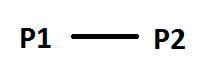
\includegraphics[width=3cm]{../Graphics/connected_nodes}

					\begin{tikzpicture}[node distance=2cm, on grid]
						\node (p1) at (0,0) {};
						\node (p2) [right of = p1] {};

						\path[every node/.style={font=\sffamily\small}]
						(p1) edge node {} (p2);

						\fill (p1) circle (0.1) node [left] {$p1$};
						\fill (p2) circle (0.1) node [right] {$p2$};


					\end{tikzpicture}

				}	\tabularnewline

		\end{tabular}
		\item[{Binding edge}] To represent variables bound together through a common variable(Bindings) we
		choose to visualize this using normal cloud notation around them.\\
		\begin{tabular}{c  c}

			$p(x) \land q(x)$ becomes &
			\raisebox{-.5\height}{

				\begin{tikzpicture}[node distance=2cm, on grid]
				\node (p1) at (0,0) {};
				\node (p2) [right of = p1] {};

				\begin{scope}[fill opacity=0.8]
				\filldraw[fill=white!70]
				($(p1)+(-0.5,-0.5)$)
				to($(p1)+(-0.5,0.5)$)
				to($(p2)+(0.5,0.5)$)
				to ($(p2)+(0.5,-0.5)$)
				to ($(p2)+(0.5,-0.5)$)
				to ($(p1)+(-0.5,-0.5)$)
				;
				\end{scope}


				\fill (p1) circle (0.1) node [left] {$p1$};
				\fill (p2) circle (0.1) node [right] {$q1$};

				\end{tikzpicture}

				}
				\tabularnewline

		\end{tabular}
	\end{description}
	\begin{figure}
		\centering
		\begin{tikzpicture}[node distance=2cm, on grid]
		\node (aA1) at (0,0) {};
		\node (aA2) [right of = aA1] {};

		\node (aB1) [above of = aA2] {};
		\node (aB2) [right of = aB1] {};


		\node (at2) [above of = aB1] {};
		\node (at1) [above of = at2] {};

		\node (sokoAt1) [above of = aB2] {};

		\node (v1) at (1.5,3) {};
		\node (v2) at (1.5,3) {};
		\node (v3) at (4,2.5) {};
		\node (v4) at (0,0) {};
		\node (v5) at (2,0.5) {};
		\node (v6) at (3.5,0) {};
		\node (v7) at (2.5,-1) {};

		\begin{scope}[fill opacity=0.8]
		\filldraw[fill=red!70]
			($(aA2)+(-0.5,-0.5)$)
			to ($(at2)+(-0.5,0.5)$)
			to ($(at2)+(0.5,0.5)$)
			to ($(aA2)+(0.5,-0.5)$)
			to ($(aA2)+(0.5,-0.5)$)
			to ($(aA2)+(-0.5,-0.5)$)
		;

		\filldraw[fill=green!70]
			($(aB2)+(-0.5,-0.5)$)
			to($(sokoAt1)+(-0.5,0.5)$)
			to($(sokoAt1)+(0.5,0.5)$)
			to ($(aB2)+(0.5,-0.5)$)
			to ($(aB2)+(0.5,-0.5)$)
			to ($(aB2)+(-0.5,-0.5)$)
		;

		\filldraw[fill=blue!70]
			($(aA1)+(-0.5,-0.5)$)
			to($(aA1)+(-0.5,0.5)$)
			to($(aA1)+(0.5,0.5)$)
			to ($(aA1)+(0.5,-0.5)$)
			to ($(aA1)+(0.5,-0.5)$)
			to ($(aA1)+(-0.5,-0.5)$)
		;

		\filldraw[fill=yellow!70]
			($(at1)+(-0.5,-0.5)$)
			to($(at1)+(-0.5,0.5)$)
			to($(at1)+(0.5,0.5)$)
			to ($(at1)+(0.5,-0.5)$)
			to ($(at1)+(0.5,-0.5)$)
			to ($(at1)+(-0.5,-0.5)$)
		;

		\end{scope}


		\path[every node/.style={font=\sffamily\small}]
			(aA1) edge node {} (aA2)
			(aB1) edge node {} (aB2)
			(at1) edge node {} (at2);

		\fill (aA1) circle (0.1) node [below] {$adj1$};
		\fill (aA2) circle (0.1) node [below] {$adj2$};

		\fill (aB1) circle (0.1) node [below] {$adj1$};
		\fill (aB2) circle (0.1) node [below] {$adj2$};

		\fill (at1) circle (0.1) node [below] {$at1$};
		\fill (at2) circle (0.1) node [below] {$at2$};

		\fill (sokoAt1) circle (0.1) node [below] {$soAt1$};



		\node at (2.3,2.8) {$y$};
		\node at (0.3,0.3) {$x$};
		\node at (4.3,2.8) {$z$};

		\node at (2.3,6.3) {$b$};
		\end{tikzpicture}

		\caption{\label{fig:ca:sokoban-hypergraph}Sokoban as hypergraph for Example \ref{ex:ca:sokoban-hypergraph}}

	\end{figure}






\begin{example}\label{ex:ca:sokoban-hypergraph}
	Consider Example \ref{ex:ca:sokoban-moveleft-action}. In this we had
	\begin{align*}
		\sigma(S_{before}, \delta) =
			\left\{
			\begin{gathered}
				\texttt{adj-h}(x, y), \\
				\texttt{adj-h}(y, z), \\
				\texttt{at}(y), \\
				\texttt{sokobanAt}(z)
			\end{gathered}
			\right\}
	\end{align*}
	When represented as a hypergraph (see \figref{fig:ca:sokoban-hypergraph}),
	we see that each binding is clearly visualized and that two of the same predicate (\texttt{adj-h}) can be in the same graph.
	Also by modelling this as a graph the idea of disproving bindings also
	becomes explicit as it literally means to remove a node from a binding edge.
	Furthermore, in this model the notion of disjoint predicates (Restriction \ref{rst:ca:no-disjuntive-conditionals}) is shown by the nodes not being connected through any type of edge.
\end{example}


\begin{proposition}
    All vertices in a hypergraph $H$ is member of exactly one predicate edge and one binding edge.
\end{proposition}

\end{document}
